\documentclass[10pt]{article}
 
\usepackage{graphicx}
\usepackage{url}
\usepackage[english]{babel}
\usepackage{vmargin} 
\setpapersize{USletter}
\setmarginsrb{1in}{1in}{1in}{1in}{40pt}{6mm}{20pt}{20mm} 

\def\msp{\def\baselinestretch{.9}\large\normalsize}
\def\ssp{\def\baselinestretch{1}\large\normalsize}
\def\hsp{\def\baselinestretch{1.5}\large\normalsize}
\def\dsp{\def\baselinestretch{2.0}\large\normalsize}

\setcounter{secnumdepth}{2}
\setcounter{tocdepth}{3}

\hyphenation{pu-bli-sh-ed}

\ssp
\begin{document}
 
\title{\textsf{Organizing an Inter-University Hacking Competition}}

\author{Giovanni Vigna, Christopher Kruegel, Darren Mutz, \\
William Robertson, and Fredrik Valeur\\ 
\\
Reliable Software Group\\
Department of Computer Science\\
University of California, Santa Barbara\\
\texttt{\{vigna,chris,dhm,wkr,fredrik\}@cs.ucsb.edu}
}


\date{}

\maketitle

\begin{abstract}
Teaching practical network security requires the use of tools and techniques
to support the educational process and to evaluate the students' newly
achieved skills. A fundamental tool that supports a hands-on approach to
network security are live exercises. ��However, live exercises are difficult
to set up and to manage. For this reason, there are very few courses that
offer live exercises as an integral part of the class work. This paper
describes an inter-institution live exercise that has been developed as part
of a graduate-level Computer Science course on network security and intrusion
detection. The exercise involved 14 teams from 7 insitution and represented a
very first instance of this kind of exercise.

  \noindent {\bf Keywords:} Teaching Security, Security Testing, Capture The Flag, Red Team/Blue Team.
\end{abstract}

\section{Introduction}
\label{introduction}


%\begin{itemize}

%	\item Teaching practical security

%	\item Why live exercise are important

%	\item Why live exercise are hard to setup and execute

%	\item Why lessons learned are important

%	\item Why scoring software is important

%\end{itemize}

Computer security has become a critical issue that affects our everyday
life. For this reason, most colleges and other educational institutions have
devoted a consistent amount of resources to develop courses and curricula that
involve security training~\cite{bishop97,bishop00}. Typical courses include
cryptography, general computer security, network security, and specialized
topics, such as firewalls, security of wireless networks, etc.  Most of these
courses are taught using standard educational tools, such as textbooks,
slides, and papers. In addition, assignment and tests are mostly paper-based
and theoretical.  In few instances, courses are characterized by a practical,
hands-on approach. These courses are seldom offered because of the additional
difficulties of teaching practical security. First of all, security permeates
a wide range of technologies. Addressing a comprehensive set of practical
security techniques without getting lost in the details of each technology
requires careful selection of the topics and particular attention to the way
the topics are presented to the students. Second, the instructor is faced with
the difficult decision of choosing the right balance between a completely
theoretical approach and a completely practical one~\cite{bishop99}. Usually,
this choice is heavily influenced by the educational curriculum. For example,
if there is an existing course that covers the foundational principles of
security (e.g., the Bell-LaPadula model), then it is possible to use the
course as a prerequisite and focus on more practical issues. Third, teaching
practical security requires substantial effort on the part of both the
instructor and the educational institution within which the course is given.
This makes it difficult to organize practical security courses, particularly
in higher education public institutions, like universities, where resources
are scarce.  In addition, if the class has a high-impact technical content
(e.g., the class covers break-in techniques), then there is a general concern
that the class may get ``out of hand'' or that a particular institution may be
flagged as a ``hacker school''~\cite{brandt03}.  Nonetheless, we advocate that
teaching practical security is important because of the critical nature of the
topic. A security education curriculum that covers only the theoretical
aspects of security and does not give the students the opportunity to
experiment in practice with security technologies cannot prepare the students
to the complexity and difficulties of doing research and development in the
computer security field.

\section{``Capture The Flag'' Exercises}

General concepts in computer science can often be described on an abstract
level where details are omitted for the sake of clarity. While abstraction is
a useful tool to convey the ``big picture'' of a problem, there is hardly any
area in computer science where details are as significant as in computer
security. After all, a security problem is often caused by a problem in a
particular implementation of a design or protocol that is without flaw on
paper. Of course, helpful classifications of security problems exist, and
these classifications help to understand similarities between
vulnerabilities. In the end, however, each bug is embedded in a different
environment and has to be understood and corrected on a case by case
basis. Therefore, we are convinced that hands-on experience, which forces
students to deal with the details of a particular computer system and its
vulnerabilities, is an integral part of teaching computer security.

The inter-university hacking competition evolved from a series of practical
exercises that were organized by Giovanni Vigna during his computer security
classes at UC Santa Barbara~\cite{vigna03:exercises,vigna03:teaching} in
previous years.

The exercises started as a red team/blue team competition where about 50
students of the graduate security class were divided into two different
teams. As is common in a red team/blue team exercise, one group (red team)
took the role of the attacker that had to break into the other group's (blue
team) host. There were two main problems with this format. One issue was that
students were forced to be on only one side, either participating on the
offense or defense. The other problem were a number of unrealistic
restrictions that had to be enforced during the exercise to keep it fair. In
order to allow the attackers to gain access to the defender's machine, the
defenders were neither allowed to block network traffic nor to disable or
patch services. The reason was that defenders were not required to offer
services and thus could have denied all access to their machine to score an
easy victory.

The following exercise attempted to address the imbalance inherent in a
traditional red team/blue team competition by having both teams take the roles
of attacker and defender. In this setup, both teams had to simultaneously
protect their own assets while trying to obtain access to the other teams'
hosts. However, it was again necessary to introduce rules that would prevent
defenders from locking down their host.

In an attempt to lift all artificial restrictions, the exercise was redesigned
to become a {\it treasure hunt}. The idea of the treasure hunt was to have two
teams break into a simulated (yet realistic) payroll system. The exercise was
organized in a series of steps that both teams had to complete before
advancing to the next task. The team that completed a particular task faster
was awarded more points. This setup was balanced because both teams had to
perform similar tasks. In addition, no restrictions were placed on the way the
steps would be accomplished. Students were put into a situation where the
mission goals were revealed piece by piece, creating an exciting exercise for
the participants involved. However, the problem from an educational point of
view was the fact that no defense was required.

In Summer 2003, we started to prepare for the exercise that would be part of
the security class in the upcoming fall quarter at UC Santa Barbara. It was
clear that the education of students was the top priority and thus the
exercise would have to include both attack and defense tasks for both
teams. Also important was to place as few restrictions as necessary on the
participants. During this time, the authors attended Defcon 11, an event that
calls itself ``the largest underground hacking event in the world''. One of
the official Defcon events with a long tradition is the {\it capture the flag
(CTF)} contest. At Defcon 11, CTF was organized by the ``Ghetto Hackers'', a
group of hackers that had won the CTF all three of the previous years.

Defcon capture the flag is a hacking contest where eight teams have to defend
their respective servers while simultaneously trying to take over other team's
machines. Each server provides a set of public services. A team receives
points on an ongoing basis for services that are both operational {\it and}
under the team's control. A neutral scorebot periodically connects to a
service and simulates honest user interaction to check its correct
functionality. During this interaction, a {\it flag} value is checked, which
is used to identify the team that controls the service. By changing this flag
value on a competitor's machine, a team can get control of a service that is
not running on its own server, and receive additional points. To prevent
bandwidth denial of service attacks, teams have to pay points for their
bandwidth usage. The team with the most points wins in the end.

The event takes place over three days and usually attracts a large crowd of
skilled hackers. Because of the skilled audience and the relatively long time
frame, it is a challenge to create a competition that remains interesting for
the duration of the contest. In addition, it is not easily possible to enforce
an extensive rule set.

The nature of this competition was appealing to us in several ways. First,
instead of creating difficult to enforce rules of conduct, the Defcon CTF
scoring system was used to discourage disruptive behavior. Second, all teams
require both good attackers and skilled defenders to compete effectively. And
third, the defenders could not disable access to their systems without locking
out the scorebot and losing scoring opportunities. These factors influenced
our decision to design our hacking competition for the upcoming security class
as a capture the flag exercise similar to the one at Defcon.

However, the Defcon CTF model could not be adopted verbatim. The biggest
difference was the fact that the focus of our exercise is on the education of
students who should acquire knowledge as part of a university course, while
the Defcon competition is run to have skilled hackers and security experts
prove their knowledge in a competitive environment. As an immediate
consequence, it is not possible to run the competition over multiple
days. Instead, our exercise has to be an event that can be completed within
several hours. Taking the preparation time into account, it was decided to
limit our actual CTF exercise to four hours.

Because of this relatively short time span, the vulnerabilities and services
had to be chosen accordingly. It is impossible for most students, who are new
to the area of computer security, to audit and understand complex programs in
a few hours and to develop working exploits for the bugs that were
found. Therefore, we decided to develop several different custom services,
which included web services (e.g., CGI scripts in Perl) and network services
(e.g., finger). These applications were short (at most a few hundred lines of
code) and contained vulnerabilities such as classic buffer overflows that had
been discussed previously in class. In addition, one existing service (a
streaming audio server) was slightly modified to suit the competition. For
more details of the vulnerabilities, please refer to Section~\ref{vulnsoft}.

In contrast to the Defcon competition, which required all participants to be
present at the location of the game, we wanted to involve security groups at
other universities to create an inter-university exercise. This made a more
elaborate network setup necessary than the one that sufficed for the original
CTF. When our hacking competition was finally held, thirteen teams from seven
US institutions were all connected over a VPN. In the case of Defcon, it was
only necessary to pull a network cable from a team's desk to the middle of the
room and connect it to a switch. Interestingly enough, even at Defcon, one or
two teams initially had problems establishing connectivity. Some connectivity
problems had to be overcome by teams in our setup as well, but overall, the
VPN worked very well. More details about the network infrastructure and its
setup can be found in Section~\ref{infrastructure}.

Another difference was the level of consideration and support that students
received in case of problems. Defcon is a harsh environment, especially
towards beginners, and the contest participants are supposed to be skilled
enough to troubleshoot their own problems. Even more, the failure to fix one's
problem usually results in public humiliation, be it from another team or from
the organizers. This attitude is acceptable for the Defcon CTF but obviously
not for a university exercise. Therefore, we provided support in setting up
the network connectivity and helped students in ``getting going'' with their
tasks. As an example of the level of the support, the start of the contest was
delayed by thirty minutes because some teams were not able to bring up their
services and connect to the VPN at the official start time. We also created an
IRC channel that was used during the contest to make hints available to the
teams. Another reason for being more considerate in case of problems is the
short duration of the exercise. While it is possible to lose an hour to fix a
certain problem and still win at Defcon, this would be impossible in a four
hour competition.

\section{Creating the Infrastructure}
\label{infrastructure}

The design of the exercise requires a fairly complicated infrastructure. Since
the teams were located at different places throughout the US, a way of routing
packets between the different sites was needed. Running the traffic over the
Internet was not a possibility for several reasons. First of all, it was
desirable to confine the competition traffic to a secure, isolated network to
decrease the likelihood that a computer not part of the exercise was hacked by
mistake. Also, an isolated network prevents outsiders from interfering with
the competition. Another drawback of running the traffic over the Internet is
that it is very easy to spoof IP addresses. A team could for instance perform
a denial of service attack on another team by sending a large amount of
traffic to the victim team. If the traffic's source address is spoofed, it
would be very hard to track down the responsible site.

\begin{figure}
\begin{center}
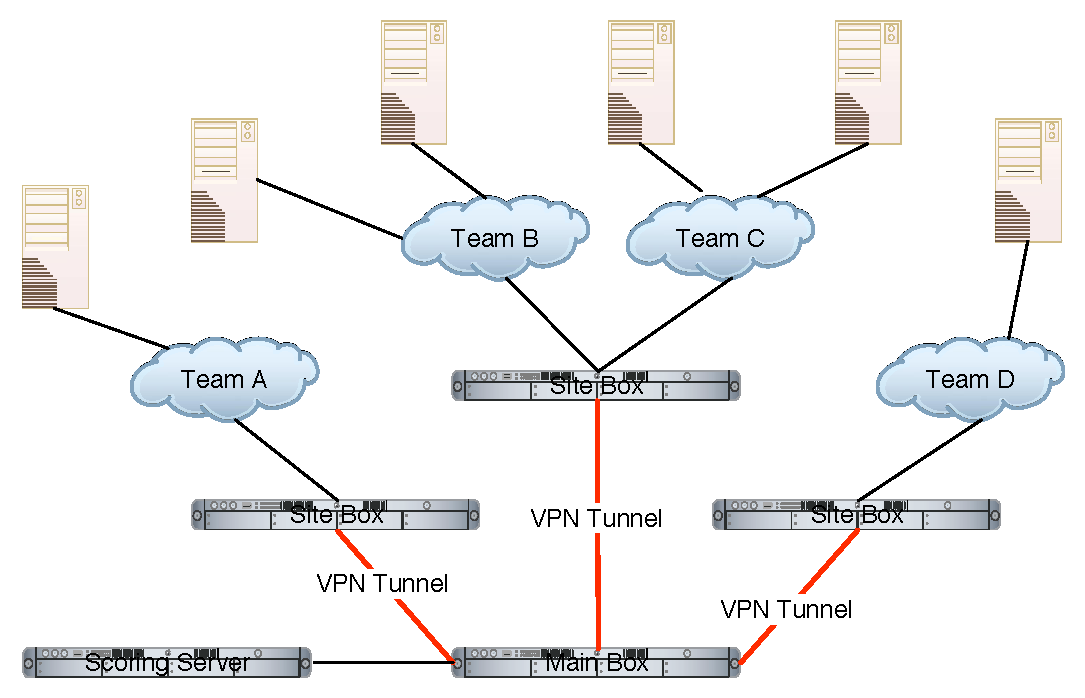
\includegraphics[width=10cm]{CTF.eps}
\end{center}
\caption{Overview of the VPN setup}
\label{vpn}
\end{figure}

In order to overcome these problems, we set up a virtual private network (VPN)
that connected all the different teams. The VPN was configured in a star
configuration as shown in Figure~\ref{vpn}. All traffic was routed through a
cental VPN server called the ``main box''. Each competition site had one VPN
gateway, called the ``site box'', which was connected to the the main box
through an encrypted tunnel. Every team at a given site had its own subnet,
which was hooked up to the respective site box. Each team connected its host
with the services to its subnetwork. In addition, each team was allowed to
connect as many extra computers to their network as they needed. These extra
computers were used for tasks such as attacking the other teams, running
intrusion detection systems, and providing a hot standby for the defending
host if it were to go down.  The scorebot, which was responsible for
calculating each team's score was hooked up to the main box to provide it with
connectivity to the tournament network. The main box and all the site boxes
were running Linux with FreeS/WAN VPN software installed. We chose FreeS/WAN
because it is free and widely available.

All traffic between the teams' subnets was routed through the main box. In
addition to forwarding the packets, the main box recorded all the traffic in
tcpdump format for later analysis. The main box also performed ingress
filtering to prevent spoofing and anonymized the traffic. Traffic anonymizing
is important because the defending teams should not be able to distinguish
traffic originating from the scorebot from traffic coming from the attacking
teams. If it is possible to identify the scorebot traffic, a packet filter
installed at the defended host could block all traffic not originating from
the scorebot and effectively prevent any team from connecting to the defended
host. The most important feature to anonymize is the source IP address. We
configured the main box to change the source address of all forwarded packets
to one specific IP address. This was accomplished by using the Linux netfilter
modules for network address translation (NAT). The main box also changed the
time-to-live (TTL) field in every packet so the teams could not identify the
source of the packet based on the number of hops the packets had
traversed. The result of the anonymizing was that all the traffic appeared to
originate from a single host.



\section{Scoring the Exercise}

Having designed the required infrastructure, the next crucial step was to
create a scoring system. Clearly, without a means of evaluating the
performance of each team, the exercise, while potentially educational in and
of itself, would quickly devolve into a convoluted mess of claimed
penetrations and misunderstandings over what constitutes a successful
defense. Thus, it was essential that a clear definition of the rules of
engagement be established.

\subsection{Scoring Concepts}

In order to create a scoring system, the first step was to define the concepts
of an available service and a successful compromise of a service. Of course,
in the real world, it is somewhat difficult to pin down an acceptable
definition for both of these ideas. For instance, it is hard to argue that
executing malicious code in the context of a remote server is not a successful
intrusion. What, however, about a remote crash or denial of service? Does an
unintended information disclosure count as an intrusion? What if the
information is relatively benign? Similarly for the case of service
availability, the inability to connect to an HTTP server is quite clearly a
sign of an unavailable service. Consider instead, however, a scenario in which
{\tt GET} and {\tt POST} requests work, but {\tt HEAD} requests fail? Is the
service available, and how does one quickly verify this? In general, verifying
the correctness of a complete software system is a hard problem, let alone
repeatedly during the course of a hacking exercise! So, as one can see, the
concepts of intrusion and availability are both in actuality quite fuzzy and
difficult to determine, and consequently a simplification was necessary in
order to reduce the problem to the realm of feasibility.

\subsubsection{Static Flags}

This simplification, borrowed from Defcon CTF events, was to utilize the
concept of a flag as a representation of service availability. A flag in this
context is defined as some feature or characteristic of a service which must
be present for the service to be considered available, and which is specific
to each service to be scored. To take a concrete example, a flag for a
database server might consist of a specific row in some table in a given
database which contains a certain value. Alternatively, for a streaming media
server, the flag might take the form of some covert channel encoded into an
audio stream. Clearly, the form the flag takes is dependent on the service,
though in order to be realistic and effective, the flag and the associated
method of checking its value must be integrated into the proper functioning of
the service in question as tightly as possible.

Given that flags are used to represent the status of a service, all the
scoring system must do to check a service is retrieve the service's flag and
check whether the value it contains is equal to the expected value, which is
simply some secret that is unique for each service for each team. If the flag
value is correct, the defending team is awarded points for successfully
providing the service for that round; otherwise, the team is not awarded
points for that round. From the attacker's perspective, a successful
penetration is performed when the attackers change the value of the service's
flag to a value associated with their team; this must typically be done by
exploiting a vulnerability in order to gain access with elevated
privileges. Thus, if the scoring system checks the defending team's flag and
finds the attacking team's flag value instead, points are awarded to the
attacking team, the defending team is not awarded points, and the service is
recorded as controlled by the attacking team. Alternatively, if a corrupted
flag is found, the defending team is awarded no points, and the service is
recorded as not available. To reset the flag so that the scorebot knows that
the service is no longer controlled by another team and that it is functioning
properly, a flag reset script is provided to each team for each service which
restores a flag to the expected value.

There are a few necessary constraints on flags and the method used to update
them. First, changing flags requires password authentication. Otherwise, there
would be no point to exploiting a vulnerability, since an attacker could
simply observe the update method used by the scoring service and apply it to
other teams. Second, the flag checks should not be conducted through
exploitation of the vulnerability present in the service so as not to reveal
their location and to allow for patching of the vulnerability without breaking
the scoring system.

A table describing the possible scoring scenarios under this system is
depicted in Table~\ref{static flag scoring table}.

\begin{table}[hptb]
\centering
\begin{tabular}{r|l}
Condition & Action \\
\hline
Defending team flag found &
  Points awarded to defending team \\
& Service recorded as available \\
\hline
Attacking team flag found &
  Points awarded to attacking team \\
& No points to defending team \\
& Service recorded as controlled by attacking team \\
\hline
Corrupt flag found &
  No points awarded to defending team \\
& Service recorded as unavailable
\end{tabular}
\caption{Static flag scoring system.}
\label{static flag scoring table}
\end{table}

This basic scoring system, while functional, is unfortunately vulnerable to
attacks which stem from the fact that service availability is now somewhat
decoupled from the ``true'' status of the service, and that flag checks can
potentially be distinguished from attack traffic. The problem is that if the
defending team is able to distinguish the scoring system's flag checks from
both normal client usage and penetration attempts from attacking teams, the
intelligent strategy would be to allow only scoring traffic and deny
everything else. Thus, the scoring system always sees a pristine flag,
attackers are unable to exploit the service to change the flag, and the
defending team smugly racks up points secure in the knowledge that they have
scammed the system. Of course, this is an unacceptable scenario, and several
techniques are used to address this. Since all traffic between teams is routed
through the main box as previously described in Section~\ref{infrastructure},
IP anonymization is utilized so that IP filtering cannot be used to firewall
off attacking systems or permit only the scoring service to connect. This
forces a defending team that persists in attempts to filter client traffic to
perform some kind of classification of client sessions on characteristics like
the structure, regularity, and frequency of requests. To address this, the
scoring system was modified to incorporate temporal check randomization,
request structure variations, as well as the inclusion of non-scoring-related
background traffic or ``chaff.'' In general, the overarching goal is to remove
(as much as possible) the ability of the defending team to distinguish scoring
traffic from other traffic.

\subsubsection{Dynamic Flags}

Related to the above issue is another potential method of distinguishing
connections from the scoring system from attacking connections.  Since it must
be assumed that a defending team can learn the locations and nature of each
flag through code analysis, sniffing network traffic, or similar means, it is
possible to watch for changes to the flag and correlate the connection that is
responsible for the change to an attacking team, since with a static flag
scoring system, only an attacking team would ever need to modify the flag
value. To address this issue, the scoring system was modified to introduce the
concept of periodic flag updates. Another idea appropriated from the Defcon
CTF, this involves periodically updating the flags for each vulnerable service
with a new value that is unfeasible to guess by both the defending and
attacking teams; this is implemented using hash chains seeded by a secret
known only to the scoring system. The use of hash chains isn't strictly
necessary, since the scoring system could simply choose a new random number
each time a new value is needed. However, using a hash chain allows for a more
robust system in the face of system crashes, as the scoring system can replay
a hash chain to resume a scoring session if necessary.

In the dynamic flag scoring system, the scoring algorithm is slightly modified
as follows. For each flag check, the flag value is first checked for
correctness as before. Assuming that the flag value is as expected, the next
value in the chain is computed and the flag is modified to contain the new
value. If, however, the flag of an attacking team is found, points are awarded
to the attackers, no points are awarded to the defenders, and the service is
recorded as controlled by the attackers. If a corrupted flag is found, the
defending team is awarded no points, and the service is recorded as
unavailable. As before, a flag reset script is provided, though in this case
the flag is set to an initial flag which is specific to each service for each
team.  The important point to note is that since the flag values for other
teams are not known, a team cannot distinguish between flag modifications
performed by an attacking team and those performed by the scoring system.

A table describing the possible scoring scenarios under the dynamic flag
scoring system is depicted in Table~\ref{dynamic flag scoring table}.

\begin{table}[hptb]
\centering
\begin{tabular}{r|l}
Condition & Action \\
\hline
Defending team initial flag found &
  Hash chain reset \\
& Flag updated to next hash chain value \\
& Service recorded as available \\
\hline
Defending team flag found &
  Points awarded to defending team \\
& Flag updated to next hash chain value \\
& Service recorded as available \\
\hline
Attacking team flag found &
  Points awarded to attacking team \\
& No points to defending team \\
& Service recorded as controlled by attacking team \\
& and flag updated to next hash chain value\\
\hline
Corrupt flag found &
  No points awarded to defending team \\
& Service recorded as unavailable
\end{tabular}
\caption{Dynamic flag scoring system.}
\label{dynamic flag scoring table}
\end{table}

However, one more problematic issue remains. Since teams know the location of
their own flags, it is a simple matter to continuously set one's flags to a
known good value. Thus, it would not matter whether attackers compromised
one's services, since the scoring system would see with a high probability the
correct flag value anyway and award service availability points. The worst an
attacker could do at this point is force a service unavailability condition,
which denies the defending team points but does not award points for a
successful compromise, effectively resulting in a stalemate. To address this,
the scoring system was slightly modified from the above to only begin awarding
points for an available service after the third round, preventing defenders to
constantly reset their flags.

\subsection{Scoring Implementation}

To implement the final scoring system design, two major components were
necessary. First, in order to retrieve and update flag values, ``get flag''
and ``set flag'' scripts needed to be created for each service. While any
underlying language or technology could be used to implement the actual
functionality required, a standard command-line interface was designed which
allowed for a uniform calling convention. For the ``get flag'' scripts, this
interface simply requires the service name and the address of a team's
server. Upon execution, the script returns the current value of the flag. The
interface is depicted in Figure~\ref{get flag interface}.

\begin{figure}[hptb]
\centering
\begin{verbatim}


    # getflag-<service name> <IP address | hostname> <password>
\end{verbatim}
\caption{``get flag'' script interface.}
\label{get flag interface}
\end{figure}

A similar interface was specified for the ``set flag'' scripts, requiring in
addition to the ``get flag'' script parameters a flag value to set and a list
of passwords to be able to write to the flag. This interface is depicted in
Figure~\ref{set flag interface}.

\begin{figure}[hptb]
\centering
\begin{verbatim}


    # setflag-<service name> <IP address | hostname> <flag value> <password>
\end{verbatim}
\caption{``set flag'' script interface.}
\label{set flag interface}
\end{figure}

The second required component of the scoring system was a centralized flag
script execution and score logging daemon, known as the scorebot.  The
scorebot is simply a daemon implemented in C++ which parses a configuration
file containing information on each team such as the team name and address of
the team server. The flag retrieval and modification scripts are provided to
the scorebot, which schedules their execution according to the previously
scoring system design, incorporating temporal randomization of flag
checks. Finally, the status of each service and point values for each team at
each round are recorded and logged to disk by the scorebot.

The current scoring system implementation is depicted in Figure~\ref{scoring
system figure}.

\begin{figure}[hptb]
\centering
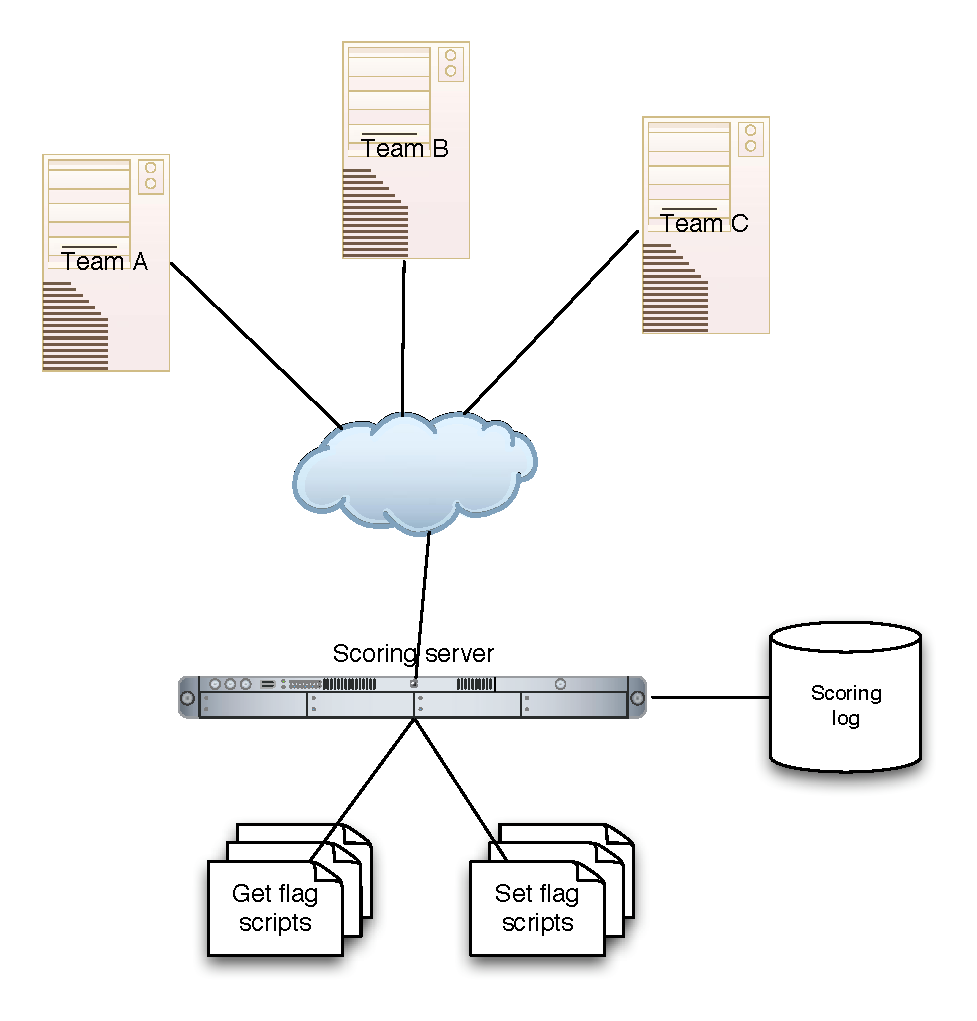
\includegraphics[scale=.5]{scoring.eps}
\caption{Current scoring system implementation.}
\label{scoring system figure}
\end{figure}


\subsection{Scoring Interface}

With the scorebot and flag management scripts in place, the scoring system was
functionally complete. Nevertheless, a critical component was still missing,
namely a graphical interface that would give some indication of each team's
performance during the competition.  To fulfill this requirement, a custom
scoreboard was created which parses the logs produced by the scorebot and
displays the current status of each team in real-time. A screenshot of the
scoreboard is shown in Figure~\ref{scoreboard}.

\begin{figure}[hptb]
\centering
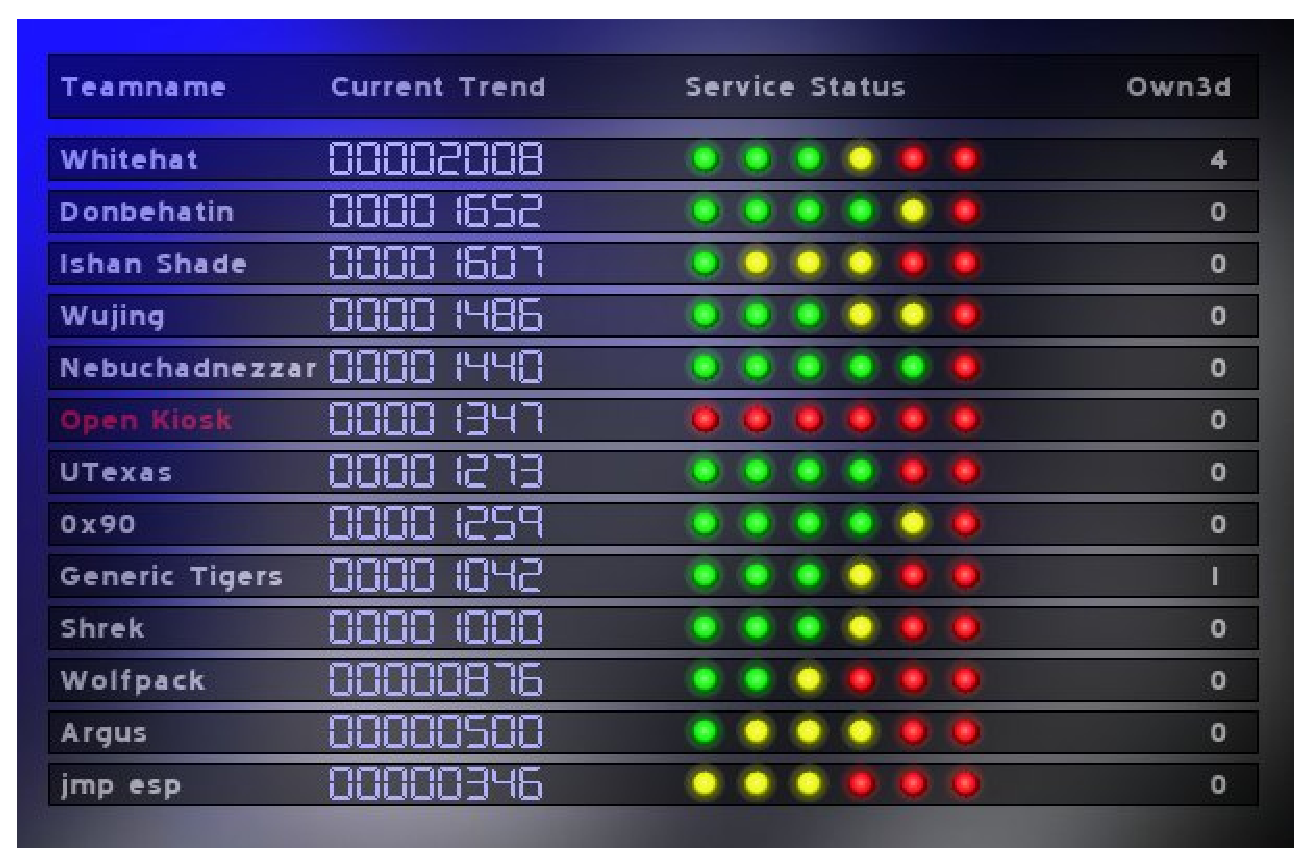
\includegraphics[scale=.5]{scoreboard.eps}
\caption{Scoreboard.}
\label{scoreboard}
\end{figure}

Each team participating in the exercise is listed in a row, along with a
numerical score and set of service status lights. Each light can be one of
green, yellow, or red. A green light indicates that a service is available and
points are awarded to {\it one} team. There is no indication of who controls
the service and it might very well be controlled by another team. We
deliberately do not distinguish the situations of having the flag controlled
by the home team or having it controlled by an attacker. This is done to
prevent people from using the scoreboard as a reliable intrusion detection
system that notifies a team of break-ins. A yellow light indicates that the
service is available but an incorrect flag is returned. That is, the flag is
neither the expected value of the current hash chain nor any teams initial
flag. A red light indicates that a service is not available at all.

The numerical score is computed as a decay function of the absolute total
score reported by the scorebot, with the intention that participants should be
given some indication of their recent performance while keeping an absolute
ranking of the teams secret. This decision was made in order to add suspense
to the competition while simultaneously providing some feedback to
participants.

The last column (``Own3d'') list the total number of services that this team
controls on other team's hosts and serves as an indication of whether attacks
are successful or not.

\section{Creating Vulnerable Software}
\label{vulnsoft}

To achieve the educational goals of this exercise -- namely, to give students
the experience of putting to use their classroom knowledge of exploiting and
correcting software vulnerabilities -- we decided to create new
vulnerabilities rather than field software with known existing security
holes. Software holes were introduced in software that was either written
completely from scratch for the contest, or added to existing software
systems. For some programs, teams were provided with the source code for the
services running on their systems from the start. For other services, source
code was provided after the first half of the exercise. Rather than measuring
a team's ability to find and apply pre-canned exploits gleaned from the
Internet, this approach has the advantage of requiring students to go through
the process of first auditing source code, then postulating avenues for
attack, developing software to exploit each vulnerability and, finally,
improving their team's defense by patching vulnerabilities in their own
software. Preserving correctness in the underlying code is critical in the
patching step, since the scorebot must be able to interact with the service in
question in order for points to be awarded.

The system given to each team consisted of a single VMware image containing a
web server and several network services. Each system had to be personalized
with respect to the initial flags associated with each service, as well as
various unique administrative passwords associated with many of the
services. With these exceptions, all images distributed to competing teams
were identical. VMware images have the additional advantage of allowing teams
to recover a known clean initial version of their system should it become
corrupted or unusable during the exercise. The remainder of this section
presents details concerning each of the services developed for the
competition.

\subsubsection{Java Servlet}

The Java servlet presents the situation in which inadequate care has been
given to security concerns in the development of a piece of in-house software
designed to interface with a backend database. In this case, the administrator
password was hardcoded into the application. While the source code was not
present on the system, the compiled byte code, in the form of a web archive,
was available for download through the web server. In order to mount an attack
on this service, students had to first locate and download the class files,
statically analyze (i.e., reverse-engineer) the Java classes to find the
authentication check, and determine the hardcoded administrator password. This
permitted the attacker access to the database and the ability to overwrite the
victim's flag with the attacking team's flag.

\subsubsection{sfind}

The sfind service was again written specifically for this exercise and
ostensibly provides remote users with the ability to search source files
stored on the server for some string. This functionality was implemented with
an invocation to the {\tt find} utility via a call to {\tt system()}. The
system was written with a standard buffer overflow vulnerability as well as a
shell escape vulnerability. Teams were able to discover this through
examination of the source code to sfind, which they were provided with.


\subsubsection{ftp}

The next service developed for this exercise was a minimal ftp server
written from scratch, which contains a classic stack buffer overflow
vulnerability. Each team was furnished with a copy of the source code
and was expected to develop a buffer overflow exploit to attack the
service.


\subsubsection{Icecast}

For this service, modifications were made to the existing open source package
Icecast, which is a streaming audio server. The idea was to simulate the
problem of Trojan code being introduced into an open source application. The
malicious code consisted of a backdoor that, if discovered in the
authentication sections of the source code, would allow a remote attacker to
issue administrative commands to the server via a web interface. The flag
setting functionality was implemented by encoding pieces of the 128-bit flag
in superfluous parameters passed to administrative commands. In order to place
their flag on the remote system, students had to first discover the backdoor
and then reverse-engineer the flag setting protocol. Some obfuscation of the
code (renaming, trivial encryption of string identifiers, application of the
{\tt lint} source code formatter) was done to make {\tt diff}'s or simple
pattern matching (e.g., via {\tt grep}) difficult; students instead needed to
read and understand the provided source code.

\subsubsection{Feedback CGI Script}

The final two services involve vulnerabilities introduced into custom
web-based common gateway interface (CGI) scripts implemented in Perl.  These
scripts were used to provide several features common to corporate web sites: a
guestbook and a feedback form.

In the case of the feedback form, examination of the source code (available on
each team's machine) reveals that one local variable used in the
authentication process is not initialized by the script. This means that the
attacker is able to set this variable to a value of her choice by passing an
appropriate CGI argument to the script. This is a commonly observed
programming error in web and PHP scripts.

\subsubsection{Guestbook CGI Script}

For the guestbook administration script, the authentication and session
tracking mechanism is implemented with cookies. Cookies are per-session values
that the server generates once and writes to each client's browser, and that
persist until the browser exits. However, in this case, the function that is
used to generate the values produces cookies with predictable values. By
analyzing the source code it is possible for the attacker to guess valid
cookies and use these guessed values to access the guestbook as an
administrator and set the service's flag to a value of her choice. The
vulnerability can be effectively removed by using a better cookie generation
function or standard packages for session management.




\section{Executing the Exercise}

The CTF was scheduled to run on December $5^{th}$ 2004 from 9 a.m. to 5
p.m. It was planned to proceed along the following three steps, having the
actual hacking contest start at 1 p.m.

\begin{enumerate}
\item Image distribution and setup.
\item Connection establishment.
\item Hacking contest.
\end{enumerate}

\subsubsection{Image Distribution and Setup} 

The VMware images, which were about 810 MByte in size, had to be distributed
to the teams prior to the start of the exercise. In order to allow for a
smooth downloading process and to prevent our server or the network from
becoming a bottleneck when all thirteen teams would attempt to download the
image from the central site at a specific point in time, the images were made
available during the night before. As mentioned above, individual images had
to be prepared separately for each team because of different flag values and
passwords. Distributing the images beforehand made sure that every team had
its image available locally at the day of the contest.

Of course, it was not possible to distribute the images directly. This would
have allowed the teams to mount the VMware partitions and study the system
prior the contest. We solved this problem by encrypting all images with the
{\tt GNU Privacy Guard}, using a shared password phrase. On the day of the
contest, at 9 a.m., the password was sent to all teams, who could now start to
decrypt and install their images. When the image was successfully loaded, the
team's next task was to make sure that the VMware image was connected to the
VPN.

\subsubsection{Connection Establishment}

As mentioned in Section~\ref{infrastructure}, each site was running a VPN
gateway. VMware makes it easy to set up a bridge mode where packets are
forwarded to the host operating system. This host machine had then to be
configured to forward packets to the VPN gateway, which was connected to the
main box at UCSB.

The main problem with the network setup and the reason for most failed
connection attempts were misconfigurations of the VPN gateways. Although teams
were provided with VMware test images and configuration files the days before
the contest, about half the teams had no connection to our scorebot at 1 a.m.,
the official start of the actual contest. We granted an additional period of
30 minutes during which the unconnected teams frantically tried to get
connected (and us providing as much troubleshooting support as possible). One
particular vicious problem was a misconfiguration that caused the ARP cache of
one of the gateway machines to fill up rapidly. This lead to a flapping link
and caused hosts on the corresponding subnet to lose and get connectivity
seemingly arbitrary. At this time, we also established an IRC channel that was
used to chat with members of other teams and to exchange tips about the setup
of the VPN. The IRC channel was later used during the actual contest to post
contest rule clarifications or to provide hints for teams in the later phases
of the competition.

At 1.30, all but one team was connected and the CTF could begin. The missing
team had a power outage at their site and it was unclear how long it would
take them to reboot and get reconnected. Therefore, it was decided to not keep
the remaining teams waiting any longer. This decision proved to be correct in
retrospect, as it took two more hours before this last team was able to join
in.

\subsubsection{Hacking Contest}

The four teams of the security class from UC Santa Barbara used the
department's two computer labs for the time of the exercise. In the main
auditorium of the computer science and engineering building, which is located
between the two computer labs, we set up our ``command center''. The command
center allowed us to stay close to our teams and was used to monitor the
network traffic that was sent over the VPN. A major component was the
scoreboard, a video projection that displayed the current scores, which were
provided by the scorebot, on a wall in the auditorium (as shown in
Figure~\ref{scoreboard}). Our students had to leave their labs and come out to
this central point to check the current status of their services and to see
the overall trend of their team's performance. Of course, the same information
was presented to all remote teams on a web page. As students were very excited
during the exercise, this focal point created a very interesting and
suspenseful atmosphere. Many people that just walked by turned into spectators
that watched the competition for a while.

In the early stage of the contest, most teams were able to keep most of their
services available. The contestants needed to familiarize themselves with the
installed software and started to look for vulnerabilities. Therefore, not
many offensive activity took place, except the scanning of other team's
networks to gather intelligence. After about one hour, the CTF reached its
first climax. The first team (which called itself {\it Whitehats}) was able to
successfully exploit a vulnerability to take over another team's service. In
retrospect, it turned out to be a decisive point in the competition. Because
no one else had found this vulnerability, the {\it Whitehats} could replicate
their attack against all other teams, controlling at some point more than
three times as many services than the second best team. While the
corresponding vulnerability was eventually found by other teams, it allowed
the {\it Whitehats} to gain a comfortably lead.

Being the first to find a vulnerability proves beneficial in two ways. First,
the services on all other hosts are not patched and the same attack can often
be mounted against many opponents. Second, there is no competition when trying
to take over other teams' vulnerable services. When several teams find the
same vulnerability, the competition for the remaining vulnerable services
significantly increases, often leading to situations where different attack
scripts continuously overwrite one flag with different values. When the number
of teams that are aware of a certain vulnerability increases, the number of
points that can be scored decreases (because less vulnerable services exist)
and, in addition, these points have to be divided among an increasing number
of attackers. In general, the number of points that can be scored by attackers
decreases rapidly when a the knowledge about a certain vulnerability becomes
more popular.

Two hours after the contest started, the source code for the two network
services {\tt sfind} and {\tt finger} was turned over to the teams. At this
point, a fierce battle for the thitherto only known vulnerable service was
raging between several teams. In the next hour, the first buffer overflows
were found in the disclosed source code. However, it was easier to patch these
bugs than to write a working exploit. Thus, when the first remote exploit was
successfully launched, only a subset of the teams were still vulnerable. In
addition, several teams developed exploits nearly simultaneously and no team
was able to take significant advantage. During the last hour, the leading
group of teams fought over the known vulnerable services, without any
significant changes in the team rankings. Eventually, the {\it Whitehats} were
successful in keeping their lead and emerged as the winners of the first
inter-university CTF that was organized at UC Santa Barbara.


\section{Lessons Learned and Future Work}

Live exercises are an important instructional tool in teaching the practical
aspects of network security.  In addition, live exercises motivate the
students to give their best because of the competitive nature of the exercise,
where the student teams success is heavily determined by the students'
creativity.

Live exercise require detailed preparation, because they are executed in a
short time span and if anything goes wrong it is difficult to solve problems
within such tight schedule.

The student feedback was overwhelmingly positive. The students of the
participating teams gave useful insights into the exercise and
enthusiastically committed to participate to next issues of the Capture The
Flag.

The next step in the evolution this exercises will be the creation of an
international Capture The Flag exercise, where teams from Universities from
around the world can participate.

For this exercise many of the lessons learned will be applied but for sure new
challenges will arise, including difference in time zone and trans-oceanic
traffic delivery.

\bibliographystyle{plain}
\bibliography{moab}

\end{document}

% LocalWords:  Vigna Darren Mutz Fredrik vigna chris dhm wkr fredrik UC backend
% LocalWords:  defender's Defcon CTF VPN IRC VMware MByte ARP moab pre
% LocalWords:  Whitehats scammed scorebot FreeS tcpdump netfilter
% LocalWords:  screenshot Servlet servlet hardcoded sfind Icecast diff grep CGI
% LocalWords:  Perl PHP Guestbook guestbook misconfigurations
